%% abtex2-modelo-trabalho-academico.tex, v-1.9.2 laurocesar
%% Copyright 2012-2017 by abnTeX2 group at http://abntex2.googlecode.com/ 
%%
%% This work may be distributed and/or modified under the
%% conditions of the LaTeX Project Public License, either version 1.3
%% of this license or (at your option) any later version.
%% The latest version of this license is in
%%   http://www.latex-project.org/lppl.txt
%% and version 1.3 or later is part of all distributions of LaTeX
%% version 2005/12/01 or later.
%%
%% This work has the LPPL maintenance status `maintained'.
%% 
%% The Current Maintainer of this work is Emílio Eiji Kavamura,
%% eek.edu@outlook.com; emilio.kavamura@ufpr.br
%% Further information about abnTeX2 are available on 
%%
%% http://abntex2.googlecode.com/
%%
%% https://code.google.com/p/abntex2/issues/ 
%%
%% Further information about UFPR abnTeX2 are available on 
%%
%% https://github.com/eekBR/ufpr-abntex/
%%
%% This work consists of the files 
% 
%          main.tex   programa principal
%      00-dados.tex   entrada de dados 
%    00-pacotes.tex   pacotes carregados no modelo
% 00-pretextual.tex   processamento dos elementos pre-textuais
%          UFPR.sty   ajusta do modelo canonico às normas  UFPR
%
%    referencias.bib
%                     e outras arquivos de imagens
%
%
%------------------------------------------------------------------------
% ------------------------------------------------------------------------
% abnTeX2: Modelo de Trabalho Academico (tese de doutorado, dissertacao de
% mestrado e trabalhos monograficos em geral) em conformidade com 
% ABNT NBR 6023:2018: Informação e documentação - Referências - Elaboração
% ------------------------------------------------------------------------
% ------------------------------------------------------------------------
%
% DATA DE ATUALIZAÇÃO: 2020-06-10

\documentclass[
% -- opções da classe memoir --
12pt,                           % tamanho da fonte
openright,                      % capítulos começam em pág ímpar (insere página vazia caso preciso)
%twoside,                        % para impressão em verso e anverso. Oposto a oneside
oneside,
a4paper,                        % tamanho do papel. 
% -- opções da classe abntex2 --
chapter=TITLE,         % títulos de capítulos convertidos em letras maiúsculas
section=TITLE,         % títulos de seções convertidos em letras maiúsculas
subsection=Title,      % títulos de subseções convertidos em letras maiúsculas
%subsubsection=TITLE,  % títulos de subsubseções convertidos em letras maiúsculas
% -- opções do pacote babel --
english,                        % idioma adicional para hifenização
%french,                         % idioma adicional para hifenização
spanish,                        % idioma adicional para hifenização
portugues,                      % o último idioma é o principal do documento
%%%%%%%%%%%%
%eek: colocação da opção para o sumario ter formatação tradicional
sumario=tradicional             % título no formato tradicional
]{abntex2}


\usepackage{UFPR}
\usepackage{enumitem}
\usepackage{float}
\usepackage{subfig}
% Pacotes básicos 
% ----------------------------------------------------------
%\usepackage{lmodern}			% Usa a fonte Latin Modern			
\usepackage[T1]{fontenc}		% Selecao de codigos de fonte.
\usepackage[utf8]{inputenc}		% Codificacao do documento (conversão automática dos acentos)
\usepackage{lastpage}			% Usado pela Ficha catalográfica
\usepackage{indentfirst}		% Indenta o primeiro parágrafo de cada seção.
\usepackage{color}		    	% Controle das cores
\usepackage{graphicx}			% Inclusão de gráficos
\usepackage{microtype} 			% para melhorias de justificação
\usepackage{ifthen}		    	% para montar condicionais
\usepackage[brazil]{babel}		% para utilizar termos em portugues
\usepackage[final]{pdfpages}    % para incluir páginas de arquivos pdf
\usepackage{lipsum}				% para geração de dummy text
\usepackage{csquotes}

%\usepackage[style=long]{glossaries}
%\usepackage{abntex2glossaries}


\usepackage{cancel} 		% permite representar o cancelamento de termos em texto ou equacoes	
\usepackage{xcolor} 		% cores extendidas	
\usepackage{smartdiagram}   	% gera diagramas a partir de listas
%\usepackage{float} 		% Para a figura ficar na posição correta	    
\usepackage{textcomp} 		% supporte para fontes da Text Companion 
\usepackage{longtable}		% uso de longtable
\usepackage{amsmath}		% simbolos matematicos
\usepackage{lscape}		% páginas em paisagem
\usepackage{multicol}		% mescla de colunas em tabelas
\usepackage{multirow}		% mescla de linhas em tabelas
\usepackage{newfloat} 		% criação do indice de quadros
%\usepackage{caption} 		% configura legenda 
	%[format=plain]
	%\renewcommand\caption[1]{%
    	%\captionsetup{font=small}	% tamanho da fonte 10pt
    	%,format=hang
 	% \caption{#1}}
	%\captionsetup{width=0.8\textwidth}
\captiondelim{-- }
\captiontitlefont{\small}
\captionnamefont{\small}

% Pacotes de citações BibLaTeX
% ----------------------------------------------------------
\usepackage[style=abnt,
	backref=true,
	backend=biber,
	citecounter=true,
	backrefstyle=three, 
	url=true,
	maxbibnames=99,
    mincitenames=1,
    maxcitenames=2,
    backref=true,
    hyperref=true,
    firstinits=true,
    uniquename=false,
    uniquelist=false]{biblatex}

% Texto padrão para as referências
% ----------------------------------------------------------
\DefineBibliographyStrings{brazil}{%
	 backrefpage  = {Citado \arabic{citecounter} vez na página},		% originally "cited on page"
	 backrefpages = {Citado \arabic{citecounter} vezes nas páginas},	% originally "cited on pages"
	 urlfrom      = {Dispon\'ivel em},
}

% Ajusta indentação de Referencias no ToC
% ----------------------------------------------------------
\defbibheading{bay}[\bibname]{%
  \chapter*{#1}%
  \markboth{#1}{#1}%
  \addcontentsline{toc}{chapter}
  {\protect\numberline{}\bibname}
}

% Formatando o avançao dos títulos no sumário 
% ----------------------------------------------------------
\makeatletter
	\pretocmd{\chapter}{\addtocontents{toc}{\protect\addvspace{-12\p@}}}{}{}
	\pretocmd{\section}{\addtocontents{toc}{\protect\addvspace{-3\p@}}}{}{}
\makeatother

% Para retirar os símbolos <> da URL  
% ----------------------------------------------------------
\DeclareFieldFormat{illustrated}{\addspace #1\isdot}%
%\DeclareFieldFormat{url}{\bibstring{urlform}\addcolon\addspace<\url{#1}>}%
%\DeclareFieldFormat{url}{\bibstring{urlfrom}\addcolon\addspace<\url{#1}>}%
\DeclareFieldFormat{url}{\bibstring{urlfrom}\addcolon \space\addspace{#1}} 
% remove <> em urls de acordo com abnt-6023:2018	

% Ajustar o espaço para a formatação da data
% ----------------------------------------------------------
\DeclareFieldFormat{urldate}{\bibstring{urlseen}\addcolon\addspace #1}%
\DeclareFieldFormat*{note}{\addspace #1}%

% Para ajustar o tamanho da fonte do número da primeira página do capítulo
% comando utilizado na parte textual 
% ----------------------------------------------------------
\makepagestyle{chapfirst}% Just for the first page of a chapter
\makeoddhead{chapfirst}{}{}{\footnotesize{\thepage}}

%%criar um novo estilo de cabeçalhos e rodapés
\makepagestyle{simplestextual}
  %%cabeçalhos
  \makeevenhead{simplestextual} %%pagina par
     {}{}{\footnotesize \thepage}
     
  \makeoddhead{simplestextual} %%pagina ímpar ou com oneside
     {}{}{\footnotesize \thepage}
  %\makeheadrule{simplestextual}{\textwidth}{\normalrulethickness} %linha
  %% rodapé
  \makeevenfoot{simplestextual}
     {}{}{} %%pagina par
      
  \makeoddfoot{simplestextual} %%pagina ímpar ou com oneside
     {}{}{}
     
% Define a formatação dos capítulos póstextuais numerados
% ----------------------------------------------------------
\newcommand{\poschap}[1]{
	\stepcounter{chapter}
	\markboth{#1}{#1}%
	\pdfbookmark[2]{#1}{#1}
	\addtocontents{toc}{\vspace{-0pt}}
	\addcontentsline{toc}{chapter}{\hspace{14.5mm}\textbf{\appendixname~
	\thechapter~- #1}}
	\chapter*{\appendixname\space\space\thechapter~- \uppercase{#1}}%
	{}
}
\newcommand{\refap}[1]{\hyperref[#1]{Apêndice~\ref{#1}}} 	% Referência apÊndices
% uso do tikz e pgfplots
% ----------------------------------------------------------
%\usetikzlibrary{external}
\usetikzlibrary{arrows,calc,patterns,angles,quotes}
\usepackage{pgfplots}
\pgfplotsset{compat=1.15}

% Define o comando para citação de fontes em elementos gráficos (figuras, imagens,...).
% ----------------------------------------------------------
%  AUTOR(ano)
%
% parâmetro é a bibkey da fonte
  
\newcommand{\citefg}[1]{~\citeauthor{#1}(\citeyear{#1})}


%%%%%%%%%%%%%%%%%%%%%%%%%%%%%%%%%%%%%%%%%%%%%%%%%%%%%%%
% Arquivo para entrada de dados para a parte pré textual
%%%%%%%%%%%%%%%%%%%%%%%%%%%%%%%%%%%%%%%%%%%%%%%%%%%%%%%
% 
% Basta digitar as informações indicidas, no formato 
% apresentado.
%
%%%%%%%
% Os dados solicitados são, na ordem:
%
% tipo do trabalho
% componentes do trabalho 
% título do trabalho
% nome do autor
% local 
% data (ano com 4 dígitos)
% orientador(a)
% coorientador(a)(as)(es)
% arquivo com dados bibliográficos
% instituição
% setor
% programa de pós gradução
% curso
% preambulo
% data defesa
% CDU
% errata
% assinaturas - termo de aprovação
% resumos & palavras chave
% agradecimentos
% dedicatoria
% epígrafe


% Informações de dados para CAPA e FOLHA DE ROSTO
%----------------------------------------------------------------------------- 
\tipotrabalho{Trabalho Acadêmico}
%    {Relatório Técnico}
%    {Dissertação}
%    {Tese}
%    {Monografia}

% Marcar Sim para as partes que irão compor o documento pdf
%----------------------------------------------------------------------------- 
 \providecommand{\terCapa}{Sim}
 \providecommand{\terFolhaRosto}{Sim}
 \providecommand{\terTermoAprovacao}{Nao}
 \providecommand{\terDedicatoria}{Nao}
 \providecommand{\terFichaCatalografica}{Nao}
 \providecommand{\terEpigrafe}{Nao}
 \providecommand{\terAgradecimentos}{Nao}
 \providecommand{\terErrata}{Nao}
 \providecommand{\terListaFiguras}{Sim}
 \providecommand{\terListaQuadros}{Sim}
 \providecommand{\terListaTabelas}{Sim}
 \providecommand{\terSiglasAbrev}{Nao}
 \providecommand{\terResumos}{Nao}
 \providecommand{\terSumario}{Sim}
 \providecommand{\terAnexo}{Nao}
 \providecommand{\terApendice}{Nao}
 \providecommand{\terIndiceR}{Nao}
%----------------------------------------------------------------------------- 

\titulo{TRABALHO ACADÊMICODE PROBABILIDADE E ESTATÍSTICA, TURMA S02}
\autor{Eduardo Augusto Andrade Chollet, Nattan Peixoto Souza,  José Moscardi da Silva Junior e Lucas Ken}
\local{Curitiba}
\data{2021} %Apenas ano 4 dígitos

% Orientador ou Orientadora
\orientador{}
%Prof Emílio Eiji Kavamura, MSc}
\orientadora{Prof\textordfeminine~Dr\textordfeminine~Silvana Heidemann, DAEST}
% Pode haver apenas uma orientadora ou um orientador
% Se houver os dois prevalece o feminino.

% Em termos de coorientação, podem haver até quatro neste modelo
% Sendo 2 mulhere e 2 homens.
% Coorientador ou Coorientadora
\coorientador{}%Prof Morgan Freeman, DSc}
\coorientadora{}

% Segundo Coorientador ou Segunda Coorientadora
\scoorientador{}
%Prof Jack Nicholson, DEng}
\scoorientadora{}
%Prof\textordfeminine~Ingrid Bergman, DEng}
% ----------------------------------------------------------
\addbibresource{referencias.bib}

% ----------------------------------------------------------
\instituicao{Universidade Tecnológica Federal do Paraná}

\def \ImprimirSetor{}%
%Setor de Tecnologia}

\def \ImprimirProgramaPos{}%Programa de Pós Graduação em Engenharia de Construção Civil}

\def \ImprimirCurso{}%
%Curso de Engenharia Civil}

\preambulo{
Trabalho  apresentado  à disciplina  Probabilidade e Estatística   (MA70H),   turma   S02,   ofertada   pelo Departamento    Acadêmico    de    Estatística,    da Universidade   Tecnológica Federal   do   Paraná, campus Curitiba, como requisito de composição da 1 nota parcial.}
%do grau de Bacharel em Expressão Gráfica no curso de Expressão Gráfica, Setor de Exatas da Universidade Federal do Paraná}

%----------------------------------------------------------------------------- 

\newcommand{\imprimirCurso}{}
%Programa de P\'os Gradua\c{c}\~ao em Engenharia da Constru\c{c}\~ao Civil}

\newcommand{\imprimirDataDefesa}{
09 de Dezembro de 2018}

\newcommand{\imprimircdu}{
02:141:005.7}

% ----------------------------------------------------------
\newcommand{\imprimirerrata}{
Elemento opcional da \cites[4.2.1.2]{NBR14724:2011}. Exemplo:

\vspace{\onelineskip}

FERRIGNO, C. R. A. \textbf{Tratamento de neoplasias ósseas apendiculares com
reimplantação de enxerto ósseo autólogo autoclavado associado ao plasma
rico em plaquetas}: estudo crítico na cirurgia de preservação de membro em
cães. 2011. 128 f. Tese (Livre-Docência) - Faculdade de Medicina Veterinária e
Zootecnia, Universidade de São Paulo, São Paulo, 2011.

\begin{table}[htb]
\center
\footnotesize
\begin{tabular}{|p{1.4cm}|p{1cm}|p{3cm}|p{3cm}|}
  \hline
   \textbf{Folha} & \textbf{Linha}  & \textbf{Onde se lê}  & \textbf{Leia-se}  \\
    \hline
    1 & 10 & auto-conclavo & autoconclavo\\
   \hline
\end{tabular}
\end{table}}

% Comandos de dados - Data da apresentação
\providecommand{\imprimirdataapresentacaoRotulo}{}
\providecommand{\imprimirdataapresentacao}{}
\newcommand{\dataapresentacao}[2][\dataapresentacaoname]{\renewcommand{\dataapresentacao}{#2}}

% Comandos de dados - Nome do Curso
\providecommand{\imprimirnomedocursoRotulo}{}
\providecommand{\imprimirnomedocurso}{}
\newcommand{\nomedocurso}[2][\nomedocursoname]
  {\renewcommand{\imprimirnomedocursoRotulo}{#1}
\renewcommand{\imprimirnomedocurso}{#2}}


% ----------------------------------------------------------
\newcommand{\AssinaAprovacao}{

\assinatura{%\textbf
   {Professora} \\ UFPR}
   \assinatura{%\textbf
   {Professora} \\ ENSEADE}
   \assinatura{%\textbf
   {Professora} \\ TIT}
   %\assinatura{%\textbf{Professor} \\ Convidado 4}
      
   \begin{center}
    \vspace*{0.5cm}
    %{\large\imprimirlocal}
    %\par
    %{\large\imprimirdata}
    \imprimirlocal, \imprimirDataDefesa.
    \vspace*{1cm}
  \end{center}
  }
  
% ----------------------------------------------------------
%\newcommand{\Errata}{%\color{blue}
%Elemento opcional da \textcite[4.2.1.2]{NBR14724:2011}. Exemplo:
%}

% ----------------------------------------------------------
\newcommand{\EpigrafeTexto}{%\color{blue}
\textit{``Não vos amoldeis às estruturas deste mundo, \\
		mas transformai-vos pela renovação da mente, \\
		a fim de distinguir qual é a vontade de Deus: \\
		o que é bom, o que Lhe é agradável, o que é perfeito.\\
		(Bíblia Sagrada, Romanos 12, 2)}
}

% ----------------------------------------------------------
\newcommand{\ResumoTexto}{%\color{blue}
Segundo a \textcite[3.1-3.2]{abntex2modelo}, o resumo deve ressaltar o  objetivo, o método, os resultados e as conclusões do documento. A ordem e a extensão destes itens dependem do tipo de resumo (informativo ou indicativo) e do tratamento que cada item recebe no documento original. O resumo deve ser precedido da referência do documento, com exceção do resumo inserido no próprio documento. (\ldots) As palavras-chave devem figurar logo abaixo do  resumo, antecedidas da expressão Palavras-chave:, separadas entre si por ponto e finalizadas também por ponto.
}

\newcommand{\PalavraschaveTexto}{%\color{blue}
latex. abntex. editoração de texto.}

% ----------------------------------------------------------
\newcommand{\AbstractTexto}{%\color{blue}
This is the english abstract.
}
% ---
\newcommand{\KeywordsTexto}{%\color{blue}
latex. abntex. text editoration.
}

% ----------------------------------------------------------
\newcommand{\Resume}
{%\color{blue}
%Il s'agit d'un résumé en français.
} 
% ---
\newcommand{\Motscles}
{%\color{blue}
 %latex. abntex. publication de textes.
}

% ----------------------------------------------------------
\newcommand{\Resumen}
{%\color{blue}
%Este es el resumen en español.
}
% ---
\newcommand{\Palabrasclave}
{%\color{blue}
%latex. abntex. publicación de textos.
}

% ----------------------------------------------------------
\newcommand{\AgradecimentosTexto}{%\color{blue}
Os agradecimentos principais são direcionados à Gerald Weber, Miguel Frasson, Leslie H. Watter, Bruno Parente Lima, Flávio de  Vasconcellos Corrêa, Otavio Real Salvador, Renato Machnievscz\footnote{Os nomes dos integrantes do primeiro
projeto abn\TeX\ foram extraídos de \url{http://codigolivre.org.br/projects/abntex/}} e todos aqueles que contribuíram para que a produção de trabalhos acadêmicos conforme as normas ABNT com \LaTeX\ fosse possível.

Agradecimentos especiais são direcionados ao Centro de Pesquisa em Arquitetura da Informação\footnote{\url{http://www.cpai.unb.br/}} da Universidade de Brasília (CPAI), ao grupo de usuários
\emph{latex-br}\footnote{\url{http://groups.google.com/group/latex-br}} e aos novos voluntários do grupo \emph{\abnTeX}\footnote{\url{http://groups.google.com/group/abntex2} e
\url{http://abntex2.googlecode.com/}}~que contribuíram e que ainda
contribuirão para a evolução do \abnTeX.

Os agradecimentos principais são direcionados à Gerald Weber, Miguel Frasson, Leslie H. Watter, Bruno Parente Lima, Flávio de Vasconcellos Corrêa, Otavio Real Salvador, Renato Machnievscz\footnote{Os nomes dos integrantes do primeiro
projeto abn\TeX\ foram extraídos de \url{http://codigolivre.org.br/projects/abntex/}} e todos aqueles que contribuíram para que a produção de trabalhos acadêmicos conforme as normas ABNT com \LaTeX\ fosse possível.
}

% ----------------------------------------------------------
\newcommand{\DedicatoriaTexto}{%\color{blue}
\textit{ Este trabalho é dedicado às crianças adultas que,\\
   quando pequenas, sonharam em se tornar cientistas.}
	}



% compila o indice
% ----------------------------------------------------------

\makeindex
% ----------------------------------------------------------
% Início do documento
% ----------------------------------------------------------
\begin{document}
% ----------------------------------------------------------
% Adequando o uppercase titulo dos elementos nas suas respectivas legendas
% Definicoes que n\~ao funcionaram quando colocados no arquivo de estilos ou de pacotes

\renewcommand{\bibname}{{REFER\^ENCIAS}}
\renewcommand{\tablename}{TABELA }
\renewcommand{\figurename}{FIGURA }
\renewcommand{\figureautorefname}{FIGURA}
\renewcommand{\tableautorefname}{TABELA}
\renewcommand{\equationname}{EQUA\c{C}\~AO~}
\renewcommand{\equationautorefname}{EQUA\c{C}\~AO~}
\renewcommand{\theenumi}{\Alph{enumi}}

% Para ajustar o tamanho da fonte do número da primeira página do capítulo
\aliaspagestyle{chapter}{chapfirst}% customizing chapter pagestyle

% ELEMENTOS PRÉ-TEXTUAIS
\makeoddhead{chapfirst}{}{}{}
% ----------------------------------------------------------
% Capa
% ----------------------------------------------------------
 \ifthenelse{\equal{\terCapa}{Sim}}{
\imprimircapa}{}

% Folha de rosto
% ----------------------------------------------------------
\imprimirfolhaderosto*

% Inserir a ficha bibliografica
% ----------------------------------------------------------
 \ifthenelse{\equal{\terFichaCatalografica}{Sim}}
 {\insereFichaCatalografica{}\cleardoublepage}
 {}

% Inserir errata
% ----------------------------------------------------------
 \ifthenelse{\equal{\terErrata}{Sim}}
 {\begin{errata}%\color{blue}
   \imprimirerrata
  \end{errata}}
 {}

% Inserir folha de aprovação
% ----------------------------------------------------------
\ifthenelse{\equal{\terTermoAprovacao}{Sim}}{
\insereAprovacao}{}

% Dedicatória
% ----------------------------------------------------------
\ifthenelse{\equal{\terDedicatoria}{Sim}}{
\begin{dedicatoria}
   \vspace*{\fill}
   \centering
   \noindent
   \DedicatoriaTexto
   \vspace*{\fill}
\end{dedicatoria}
}{}

% Agradecimentos
% ----------------------------------------------------------

 \ifthenelse{\equal{\terAgradecimentos}{Sim}}
 {\begin{agradecimentos}
    \AgradecimentosTexto
  \end{agradecimentos}
  }{}
% Epígrafe
% ----------------------------------------------------------

\ifthenelse{\equal{\terEpigrafe}{Sim}}{
\begin{epigrafe}
    \vspace*{\fill}
	\begin{flushright}
        \EpigrafeTexto
	\end{flushright}
\end{epigrafe}
}{}

% RESUMOS
% ----------------------------------------------------------
% resumo em português
%\setlength{\absparsep}{18pt} % ajusta o espaçamento dos parágrafos do resumo
 \ifthenelse{\equal{\terResumos}{Sim}}{
\begin{resumo}
    \ResumoTexto
    
    %\vspace{\onelineskip}
    \noindent 
    \textbf{Palavras-chaves}: \PalavraschaveTexto
\end{resumo}

%% resumo em inglês
\begin{resumo}[ABSTRACT]
 \begin{otherlanguage*}{english}
   \AbstractTexto
   
   %\vspace{\onelineskip}
   \noindent 
   \textbf{Key-words}: \KeywordsTexto
 \end{otherlanguage*}
\end{resumo}


% resumo em francês 
\ifthenelse{\equal{\Resume}{}}
{}
{
 \begin{resumo}[RESUME]%Résumé
  \begin{otherlanguage*}{french}
     \Resume
     
     %\vspace{\onelineskip}
     \noindent      
     \textbf{Mots clés}: \Motscles
  \end{otherlanguage*}
 \end{resumo}
} 

% resumo em espanhol
\ifthenelse{\equal{\Resume}{}}{}
{ \begin{resumo}[RESUMEN]
  \begin{otherlanguage*}{spanish}
    \Resumen 
   
   %\vspace{\onelineskip}
   \noindent    
    \textbf{Palabras clave}: \Palabrasclave
  \end{otherlanguage*}
 \end{resumo}
}
}{}

% inserir lista de ilustrações
% ----------------------------------------------------------
\ifthenelse{\equal{\terListaFiguras}{Sim}}{
%\pdfbookmark[0]{\listfigurename}{lof}
\listoffigures*
\cleardoublepage
}{}

% inserir lista de quadros
% ----------------------------------------------------------
\ifthenelse{\equal{\terListaQuadros}{Sim}}{
%\pdfbookmark[0]{\listtablename}{lot}
\listofquadros*
\cleardoublepage
}{}

% inserir lista de tabelas
% ----------------------------------------------------------
\ifthenelse{\equal{\terListaTabelas}{Sim}}{
%\pdfbookmark[0]{\listtablename}{lot}
\listoftables*
\cleardoublepage
}{}


% inserir lista de abreviaturas e siglas 
% inserir lista de símbolos
% ----------------------------------------------------------

 \ifthenelse{\equal{\terSiglasAbrev}{Sim}}{
    \imprimirlistadesiglas
    \cleardoublepage
    \imprimirlistadesimbolos
    \cleardoublepage
 }{}

% inserir o sumario
\makeoddhead{chapfirst}{}{}{}
% ----------------------------------------------------------
\ifthenelse{\equal{\terSumario}{Sim}}{
%\pdfbookmark[0]{\contentsname}{toc}
\tableofcontents*
%\cleardoublepage
}{}
 

 
 


% ----------------------------------------------------------
% ELEMENTOS TEXTUAIS
% ----------------------------------------------------------
\textual % \pagestyle{textualUFPR}

\pagestyle{simplestextual}
% sugerido por Youssef Cherem 20170316
% https://mail.google.com/mail/u/0/?tab=wm#inbox/15ad3fe6f4e5ff1f

% Introdução (exemplo de capítulo sem numeração, mas presente no Sumário)
% ----------------------------------------------------------
%\chapter[INTRODUÇÃO]{INTRODUÇÃO}
%---------------------------------------------------------------------------------------


\cite{ISO5122:1979}

\textcite{ISO5122:1979}

\begin{itemize}
 \item para inserir uma sigla: 
    \verb|\criarsigla|\{ABNT\}{Associa\c{c}\~ao Brasileira de Normas T\'ecnicas}:

    \criarsigla{ABNT}{Associa\c{c}\~ao Brasileira de Normas T\'ecnicas}

\item para inserir s\'imbolo: 
    \verb|\criarsimbolo{$ \Gamma $}{Letra grega Gama}|
  
    $ \Gamma $ \criarsimbolo{$ \Gamma $}{Letra grega Gama}

\end{itemize}

% Usado para testar o formato uppercase dos t\'itulos 
% em maiusculas nas respectivas listas
%---------------------------------------------------------------------------------------
\begin{table}[!ht]
 \centering
 \par\caption{TesTANDO TABELAS}

\begin{tabular}{c|c|c}
 teste1&teste1&teste1\\\hline\hline
  1&2&3\\\hline
 \end{tabular}
 \label{tab:tab01}
\end{table}



\tabela{tabela teste} %1 Título da tabela
{
\begin{tabular}{c|c|c|c|c|c}
 teste1&teste2&teste3&teste1&teste2&teste3\\\hline\hline
  1&2&3&4&5&6\\\hline
 \end{tabular}
} %2 Tabela
{\textcite{ISO5122:1979}}%3 Fonte da tabela
{teste1} %4 Label da tabela tab:teste1
{ Nota de teste } %5 Nota da tabela
{testando as figuras e tabelas, fda} %6 Legenda da tabela


\figura
{TESTE DE FIGURAS 2} %1 Legenda
{.55} %2  % da largura da área de texto
{fig/figure} %3 localização da figura
{\textcite[1]{abntex2modelo}} %4 fonte da figura
{teste} %5 etiqueta
{\url{https://goo.gl/EKFRak} TESTE DE FIGURAS 2 TESTE DE FIGURAS 2 TESTE DE FIGURAS 2 TESTE DE FIGURAS 2 TESTE DE FIGURAS 2 TESTE DE FIGURAS 2 TESTE DE FIGURAS 2 TESTE DE FIGURAS 2 TESTE DE FIGURAS 2 TESTE DE FIGURAS 2 TESTE DE FIGURAS 2} %6 Nota da figura
{} %7 Legenda da figura

\figura
{TESTE DE FIGURAS 3} % Legenda
{.65} % % da largura da área de texto
{fig/tipog} % localização da figura
{o Autor (2017)} % fonte da figura
{tipo1} % etiqueta
{}
{}

\figura
{Figura original} % Legenda
{.35} % % da largura da área de texto
{fig/fig} % localização da figura
{\textcite{luminaria01}} % fonte da figura
{tipo2} % etiqueta
{}
{}

\figurac
{Figura aparada} % Legenda
{.35} % % da largura da área de texto
{fig/fig} % localização da figura
{\textcite{luminaria01}} % fonte da figura
{tipo3} % etiqueta =>  fig:tipo3
{notinha}   % Nota
{legendonha} % legenda
{70} % laterais mm
{80} % superior e inferior mm


A \autoref{fig:teste} apresenta o seguinte detalhe que deve ser observado em pacientes com Wordnite

%---------------------------------------------------------------------------------------
\chapter{REVISÃO TEÓRICA}

\textcite[3.1-3.2]{abntex2modelo}

\textcite{luminaria01}

\textcite{luminaria01}


\textcite{luminaria01}



\textcite{luminaria01}

\textcite{ISO5122:1979}

\section{Modelo}

\subsection{Modelo simplificado}
\newpage
\textcite[3.1-3.2]{abntex2modelo}

\subsubsection{Modelo simplificadíssimo}


\chapter{Lista de Exercícios 1}


\begin{enumerate}[label=\emph{\arabic*})]

	\item Considere o material denominado "Exemplo de Relatório Estatístico – Estatística Descritiva"

	  	  Para os estudantes da disciplina Probabilidade e Estatística (MA70H), turma S09, o censo apurado para a variável "quantidade de disciplinas matriculadas no semestre letivo 2/2020" foi: 8, 5, 5, 7, 9, 7, 8, 9, 6, 8, 6, 6, 7, 7, 4, 3.

	      A turma S09 tem 20 estudantes matriculados em MA70H, mas o levantamento de dados foi feito em apenas 16 estudantes, pois um estudante chegou atrasado à aula de 24/02, quando foi realizado o levantamento de dados, e outros três estudantes não compareceram à aula de 24/02.

	      \begin{enumerate}[label=\emph{\alph*})]

		      \item Classifique a variável;
		      
				\textbf{Resolução:}	A variável é quantitativa discreta

		      \item Identifique a unidade de medida da variável;
		      
				\textbf{Resolução:}	número de disciplinas matriculadas
				
  			  \item Identifique a escala de medição da variável;
  			  
				\textbf{Resolução:}	A variável possui escala de proporcionalidade  
			  
			  \item \label{item_graficos} Para o censo acima, construa as tabelas 1, 2, 3 e 4 e os gráficos 1, 2, 3, 4 e 5, presentes no material acima referido. Não se esqueça de colocar título completo e fonte em cada tabela e em cada gráfico; caso necessário, colocar notas e chamadas no rodapé das tabelas e gráficos;
			  
				\textbf{Resolução:}
			  
			  \begin{table}[]
			  	\centering
			  	\caption{Estudantes da disciplina Probabilidade e Estatística (MA70H), turma S09, semestre  letivo  2/2020, da  Universidade  Tecnológica  Federal  do  Paraná, campus Curitiba, segundo a quantidade de disciplinas matriculadas}
			  	\resizebox{0.7\textwidth}{!}{%
			  		\begin{tabular}{cc}
			  			\hline
			  			\multicolumn{1}{c|}{Estudante} & Nº de disciplinas matriculadas \\
			  			\hline
			  			1 	& 8 \\
			  			2 	& 5 \\
			  			3 	& 5 \\
			  			4 	& 7 \\
			  			5 	& 9 \\
			  			6 	& 7 \\
			  			7 	& 8 \\
			  			8 	& 9 \\
			  			9 	& 6 \\
			  			10 	& 8 \\
			  			11 	& 6 \\
			  			12 	& 6 \\
			  			13 	& 7 \\
			  			14 	& 7 \\			  			
			  			15 	& 4 \\
			  			16 	& 3 \\
			  			17 	& Não informado, pois não participou da da aula \\
			  			18 	& Não informado, pois chegou atrasado na aula \\
			  			19 	& Não informado, pois chegou atrasado na aula \\
			  			20	& Não informado, pois chegou atrasado na aula \\
			  			\hline
			  		\end{tabular}			      
			  	}
			  	\label{tab:d-1}
			  	\begin{minipage}{0.7\linewidth}
			  		\emph{Fonte: Autoria própria}
			  	\end{minipage}	  	
			  \end{table}	  
			  
			  \begin{table}[]
			  	\centering
			  	\caption{Estudantes da disciplina Probabilidade e Estatística (MA70H), turma S09, semestre  letivo  2/2020,  da  Universidade  Tecnológica  Federal  do  Paraná, campus Curitiba, segundo a quantidade de disciplinas matriculadas}
			  	\resizebox{0.7\textwidth}{!}{%
			  		\begin{tabular}{cc}
			  			\hline
			  			\multicolumn{1}{c|}{Nº de disciplinas matriculadas} & Frequência \\
			  			\hline
			  			3 & 1 \\
			  			4 & 1 \\
			  			5 & 2 \\
			  			6 & 3 \\
			  			7 & 4 \\
			  			8 & 3 \\
			  			9 & 2 \\
			  			\hline
			  			Total & 16 \\
			  			\hline
			  		\end{tabular}			      
			  	}
			  	\label{tab:d-2}
			  	\begin{minipage}{0.7\linewidth}
			  		\emph{Fonte: Autoria própria}
			  	\end{minipage}	  	
			  \end{table}
			  
			  \begin{table}[]
			  	\centering
			  	\caption{Medidas   estatísticas   para   descrever   os   estudantes   da   disciplina Probabilidade   e   Estatística   (MA70H),   turma   S09,   semestre   letivo   2/2020,   da Universidade Tecnológica Federal do Paraná, campus Curitiba, segundo a quantidade de disciplinas matriculadas}
			  	\resizebox{0.7\textwidth}{!}{%
			  		\begin{tabular}{ccc}
			  			\hline
			  			\multicolumn{1}{c|}{Medida estatística} & \multicolumn{1}{c|}{Valor calculado} & Unidade de medida \\ \hline
			  			\multicolumn{1}{c|}{Quantidade de dados ($N$)} 				& 16 		& - 				\\
			  			\multicolumn{1}{c|}{Mínimo ($Min$)} 						& 3 		& disciplina	 	\\
			  			\multicolumn{1}{c|}{Máximo ($Max$)} 						& 9 		& disciplina		\\
			  			\multicolumn{1}{c|}{Amplitude ($A$)} 						& 6 		& disciplina 		\\
			  			\multicolumn{1}{c|}{Moda ($Mo$)} 							& 7 		& disciplina		\\
			  			\multicolumn{1}{c|}{Percentil 10 ($P_{10}$)} 				& 3 		& disciplina		\\
			  			\multicolumn{1}{c|}{Primeiro Quartil ($Q_{1}$)}			 	& 3 		& disciplina		\\
			  			\multicolumn{1}{c|}{Mediana ($\tilde{x}$)} 					& 5 		& disciplina		\\
			  			\multicolumn{1}{c|}{Terceiro Quartil ($Q_{3}$)} 			& 7 		& disciplina		\\
			  			\multicolumn{1}{c|}{Percentil 90 ($P_{90}$)} 				& 9			& disciplina		\\ 
			  			\multicolumn{1}{c|}{Média ($\mu$)} 							& 6.5625 	& disciplina		\\ 
			  			\multicolumn{1}{c|}{Variância populacional ($\sigma^{2}$)} 	& 2.929167	& disciplina$_{2}$	\\
			  			\multicolumn{1}{c|}{Desvio padrão populacional ($\sigma$)}	& 1.711481	& disciplina \\				
			  			\multicolumn{1}{c|}{Coeficiente de variação ($CV$)}			& 26.07971	& \% 				\\
			  			\multicolumn{1}{c|}{Coeficiente de assimetria ($As$)}		&-0.4393908 & -					\\			  						  			
			  			\multicolumn{1}{c|}{Coeficiente de curtose ($K$)}			&-0.5138676 & - 				\\ \hline
			  		\end{tabular}%
			  	}
			  	\label{tab:d-3}
			  	\begin{minipage}{0.7\linewidth}
			  		\emph{Fonte: Autoria própria}
			  	\end{minipage}	  	
			  \end{table}  

			  \begin{table}[]
			  	\centering
			  	\caption{Escores  padronizados  para  a  quantidade  de  disciplinas  matriculadas referente  aos  estudantes  da  disciplina  Probabilidade  e  Estatística  (MA70H),  turma S09, semestre letivo 2/2020, da Universidade Tecnológica Federal do Paraná, campus Curitiba}
			  	\resizebox{0.7\textwidth}{!}{%
			  		\begin{tabular}{ccc}
			  			\hline
			  			\multicolumn{1}{c|}{\begin{tabular}[c]{@{}c@{}}N°  de disciplinas matriculadas\\ $(X)$\end{tabular}} & \multicolumn{1}{c|}{Frequência} & \begin{tabular}[c]{@{}c@{}}Escore padronizado z, com\\ $Z_{i}=\frac{x_{i}-\mu}{\sigma}$\end{tabular} \\ \hline
			  			3 		& 1 	& -2.0815308 \\
			  			4 		& 1 	& -1.4972414 \\
			  			5 		& 2 	& -0.9129521 \\
			  			6 		& 3 	& -0.3286628 \\
			  			7 		& 4 	& 0.2556266 \\
			  			8 		& 3 	& 0.8399159 \\
			  			9 		& 2 	& 1.4242053 \\ \hline
			  			Total 	& 16 	&  \\ \cline{1-2}
		  			\end{tabular}%	  			      
			  	}
			  	\label{tab:d-4}
				\begin{minipage}{0.7\linewidth}
					\emph{Fonte: Autoria própria}
				\end{minipage}	  	
			  \end{table}
			  
			  \begin{figure}[H]
			  	\centering
			  	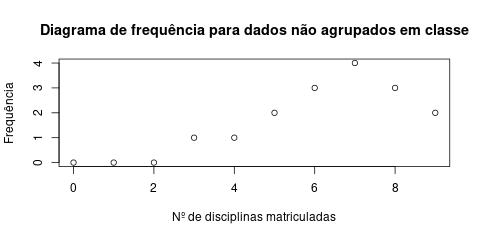
\includegraphics[width=0.7\linewidth]{fig/d-graph-3}
			  	\caption{
			  		Estudantes da disciplina Probabilidade e Estatística (MA70H), turma S09, semestre  letivo  2/2020,  da  Universidade  Tecnológica  Federal  do  Paraná, campus Curitiba, segundo a quantidade de disciplinas matriculadas
			  	}
			  	\label{fig:d-graph-3}
				\begin{minipage}{0.7\linewidth}
					\emph{\textbf{Fonte:} Autoria própria}
				\end{minipage}
			  \end{figure}	
			  
			  \begin{figure}[H]
			  	\centering
			  	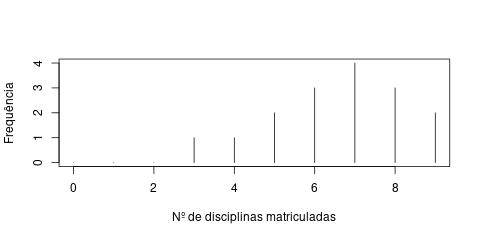
\includegraphics[width=0.7\linewidth]{fig/d-graph-4}
			  	\caption{
					Estudantes da disciplina Probabilidade e Estatística (MA70H), turma S09, semestre  letivo  2/2020,  da  Universidade  Tecnológica  Federal  do  Paraná, campus Curitiba, segundo a quantidade de disciplinas matriculadas
			  	}
			  	\label{fig:d-graph-4}
				\begin{minipage}{0.7\linewidth}
					\emph{\textbf{Fonte:} Autoria própria}
				\end{minipage}
			  \end{figure}		
			  
			  \begin{figure}[H]
			  	\centering
			  	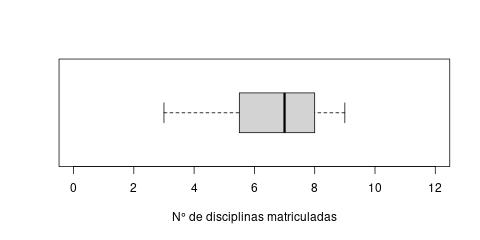
\includegraphics[width=0.7\linewidth]{fig/d-graph-5}
			  	\caption{
					Medidas   estatísticas   para   descrever   os   estudantes   da   disciplina Probabilidade   e   Estatística   (MA70H),   turma   S09,   semestre   letivo   2/2020,   da Universidade Tecnológica Federal do Paraná, campus Curitiba, segundo a quantidade de disciplinas matriculadas
		  		}
			  	\label{fig:d-graph-5}
				\begin{minipage}{0.7\linewidth}
					\emph{\textbf{Fonte:} Autoria própria}
				\end{minipage}
			  \end{figure}			  	  			  
			  
			  \item Interprete os dados e escreva uma conclusão sobre eles, baseando-se nas tabelas e gráficos construídos no item \ref{item_graficos};
			  
			  \item Fazer capa e folha de rosto nas normas de apresentação de trabalhos acadêmicos. 				  

	      \end{enumerate}	

\end{enumerate}







% PARTE DA PREPARAÇÃO DA PESQUISA
% ----------------------------------------------------------
%\part{Preparação da pesquisa}
%\input{cap02}
%

% PARTE DOS REFERENCIAIS TEÓRICOS
% ----------------------------------------------------------
%\part{Referenciais teóricos}
%\input{cap03}

% PARTE DOS RESULTADOS
% ----------------------------------------------------------
%\part{Resultados}
%\input{cap05}

% Finaliza a parte no bookmark do PDF
% para que se inicie o bookmark na raiz
% e adiciona espaço de parte no Sumário
% ----------------------------------------------------------
%\phantompart

% ---
% Conclusão (outro exemplo de capítulo sem numeração e presente no sumário)
% ---
%\chapter*[Conclusão]{Conclusão}
%\addcontentsline{toc}{chapter}{Conclusão}
% ---
%\input{cap06}

% ELEMENTOS PÓS-TEXTUAIS
% ----------------------------------------------------------
\postextual

% Ajuste vertical do titulo de referencias no sumário
% ----------------------------------------------------------
\addtocontents{toc}{\vspace{-24pt}}

% Referências bibliográficas
% ----------------------------------------------------------
%\bibliography{referencias}

\printbibliography[heading=bay]
% ----------------------------------------------------------

% Ajuste vertical dos titulos dos capitulos postextuais
% ----------------------------------------------------------
\addtocontents{toc}{\vspace{-12pt}}

% Glossário
% ----------------------------------------------------------
% Consulte o manual da classe abntex2 para orientações sobre o glossário.
%
%\glossary

% Apêndices
% ----------------------------------------------------------
\ifthenelse{\equal{\terApendice}{Sim}}
{\begin{apendicesenv}

		% Numeração arábica para os apêndices
		% --------------------------------------------------
		\renewcommand{\thechapter}{\arabic{chapter}}
		% Imprime uma página indicando o início dos apêndices
		% \partapendices

		% Existem várias formas de se colocar anexos.
		% O exemplo abaixo coloca 2 apêndices denominados de 
		% DESENVOLVIMENTO DETALHADO DA PINTURA e 
		% ESCOLHA DO MATERIAL DE IMPRESSÃO:
		% ---
		% --- insere um capítulo que é tratado como um apêndice
		%\chapter{DESENVOLVIMENTO DETALHADO DA PINTURA}
		% 
		%\lipsum[29] % gera um parágrafo
		%
		% --- insere um capítulo que é tratado como um apêndice
		%\chapter{ESCOLHA DO MATERIAL DE IMPRESSÃO}
		% 
		%\lipsum[30] % gera um parágrafo

		% --- Insere o texto do arquivo ap01.tex
		% 
		% --- O conteúdo do arquivo pode ser vários anexos ou um único apêndices.
		%     A vantagem de se utilizar este procedimento é de suprimi-lo
		%     das compilações enquanto se processa o resto do documento.

		   % --- insere um capítulo que é tratado como um apêndice
   \label{ap:ap01}
   \poschap{ESCOLHA DO MATERIAL - colocado no apendice}
    
   \lipsum[30] % gera um parágrafo
   \section*{Testes se\c{C}\~aO}

    \lipsum[22] % gera um parágrafo
	
	\poschap{ESCOLHA DO MATERIAL DE IMPRESSÃO- colocado no apendice}
    \lipsum[32] % gera um parágrafo


	\end{apendicesenv}
}{}


% Anexos
% ----------------------------------------------------------
\ifthenelse{\equal{\terAnexo}{Sim}}{
	\begin{anexosenv}

		% Numeração arábica para os apêndices
		% --------------------------------------------------
		\renewcommand{\thechapter}{\arabic{chapter}}
		% --- Imprime uma página indicando o início dos anexos
		% \partanexos

		% Existem várias formas de se colocar anexos.
		% O exemplo abaixo coloca 2 anexos denominados de 
		% TABELA DE VALORES e GRÁFICOS DE BALANCEMANTO:
		% ---
		% --- insere um capítulo que é tratado como um anexo
		%\chapter{TABELAS DE VALORES}
		% 
		%\lipsum[31] % gera um parágrafo
		%
		% --- insere um capítulo que é tratado como um anexo
		%\chapter{GRÁFICOS DE BALANCEAMENTO}
		% 
		%\lipsum[32] % gera um parágrafo

		% --- Insere o texto do arquivo ax01.tex
		% 
		% --- O conteúdo do arquivo pode ser vários anexos ou um único anexo.
		%     A vantagem de se utilizar este procedimento é de suprimi-lo
		%     das compilações enquanto se processa o resto do documento.

		   % --- insere um capítulo que é tratado como um apêndice
   \poschap{anexando ESCOLHA DO MATERIAL}
    
   \lipsum[30] % gera um parágrafo
    \section*{anexando testes secao}
    

\poschap{anexando ESCOLHA DO MATERIAL DE IMPRESSÃO}
    
   \lipsum[32] % gera um parágrafo

	\end{anexosenv}
}{}

% INDICE REMISSIVO
%---------------------------------------------------------------------
\ifthenelse{\equal{\terIndiceR}{Sim}}{
	\phantompart
	\printindex
}{}

\end{document}
